% !TEX root=/home/tavant/these/manuscript/src/manuscript.tex

% \FloatBarrier
\section{Sheath model with polytropic electrons and electron emission}
\label{sec-fluid_poly_see}

\subsection{Definition of the sheath equation} \label{subsec-def_sheat_see}

We have seen in \cref{sec-PIC_poly} that in the presence of electron emission from the wall, the electrons can be described using a polytropic state law.
The value of the polytropic index obtained from the mean electron density and temperature is for $\crover \geq 40 \,\volt$ is $\gamma = 1.35$.
Using the electron distribution function, the evolution of the forward electron seems to follow a polytropic low of index $\gamma=1.28$.
Hence, we modify the polytropic sheath model of \cref{sec-fluid} to take into account the electron emission from the wall.
This modifies the current equality at the wall to
\begin{equation} \label{eq-see-J_eq}
  \Gamma_i = (1 - \rate) \Gamma_e.
\end{equation}

Using \cref{eq-gi,eq-ge,eq-tew} for $\Gamma_i$ and $\Gamma_e$, we obtain the equality
\begin{equation}\label{eq-sheathsee}
  (1 - \rate )\left[ 1 +\frac{\gamma -1}{\gamma} \frac{ \dphi_0}{ \Te_0}  \right]^{\frac{1}{\gamma - 1}} \sqrt{1 - \frac{\gamma -1}{\gamma}\frac{\dphi_0}{\Te_0}} = \sqrt{\frac{4 \gamma \pi m_e}{m_i}}
\end{equation}

Similarly to the case without electron emission in \cref{sec-fluid}, \cref{eq-sheathsee} cannot be solved analytically, but it can be solved numerically.
The solution for $\rate=0.8$ is compared to the case without electron emission ($\rate=0$) for a \ac{Xe} plasma in \cref{fig-dphi_see}.
As expected, the potential difference decreases with increasing $\rate$.
However, the gap between the two cases decreases when $\gamma$ increases from 1 to 2.

\begin{figure}[hbtp]
  \centering
  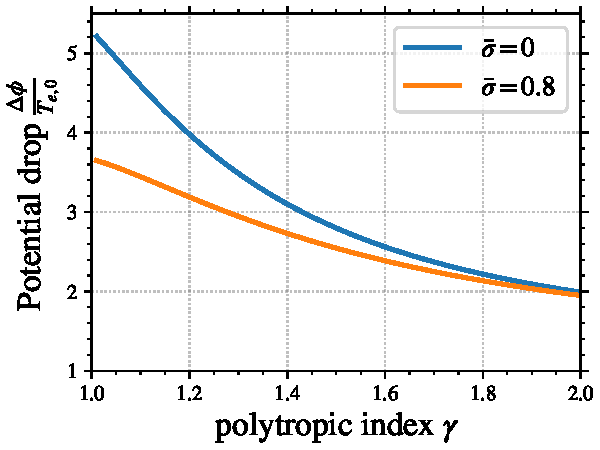
\includegraphics[width=\defaultwidth]{Sheath_drop_with_SEE.pdf}
  \caption{Potential drop $\dphi$ normilized by the bulk electron temperature $\Te_0$ as a function of the polytropic index $\gamma$ for a xenon plasma ($m_i = 131\,\atomicmass$). The emission rate $\rate$ is fixed for clarity.}
  \label{fig-dphi_see}
\end{figure}

The electron emission rate is a function of the electron energy at the wall.
Using the same hypothesis as in \cref{eq-ge}, we can define the emission rate from \cref{eq-seemaxw} by
\begin{equation} \label{eq-seemaxw_poly}
  \rate = \ratemaxw(\Tew) = \sigo + ( 1 - \sigo) \frac{ 2 \Tew  }{\crover}.
\end{equation}
Combined with \cref{eq-tew}, we obtain

\begin{equation} \label{eq-seemaxw_Tew}
  \rate = \sigo + ( 1 - \sigo) \frac{ 2 \lp \Teb - \frac{\gamma - 1}{\gamma} \dphi \rp }{\crover}.
\end{equation}
Here, for sake of clarity we do not write the saturation of $\rate$ to $\ratecr$ due to the \ac{SCL} regime.
Indeed, we know that it  changes only slightly the value of $\rate$.
%However, we include it the the next calculations.


Noting $\chi = \frac{\gamma -1}{\gamma} \frac{ \dphi_0}{ \Te_0} $, we finely obtain the equation to be solved
\begin{equation} \label{eq-costseepoly}
  \left[ 1 + \chi  \right]^{\frac{1}{\gamma - 1}} \sqrt{1 - \chi} - \frac{  \sqrt{4 \gamma m_e / m_i}}{  (1 - \sigo) [1 - \frac{2 \Teb}{\crover} (1 - \chi ) ] } = 0.
\end{equation}

\Cref{eq-costseepoly} depends explicitly on $\Teb$, hence $\chi$ is no longer independent of $\Teb$.
This adds a free parameter when solving the sheath equation.
Moreover, the \ac{LHS} of \cref{eq-costseepoly} is more complex than before, leading to multiple solutions.
\Cref{fig-costfunction} shows the \ac{LHS} of \cref{eq-costseepoly} for several values of ({\bf a}) $\Teb$ and ({\bf b}) $\crover$, while keeping the polytropic index to $\gamma=1.35$.
The \ac{SCL} regime has been taken into account by saturating $\rate$ to $\ratecr=0.982$. 
It corresponds to the branch which crosses the abscissa axis close to $\frac{\dphi}{\Teb}=1$. 


\renewcommand\subfigurewidth{0.4\textwidth}

\begin{figure}[hbtp]
  \centering
  \begin{tabular}{c c}
    \subfigure{cost_function_bis.pdf}{a}{20,20} &
    \subfigure{cost_function_2bis.pdf}{b}{20,20} \\
  \end{tabular}
  \caption{Value of the \ac{LHS} of \cref{eq-costseepoly}, labelled cost function, for several values of ({\bf a}) $\Teb$ and ({\bf b}) $\crover$.}
  \label{fig-costfunction}
\end{figure}

We can see that \cref{eq-costseepoly} can present one or three solutions, depending on the relative values of $\crover$ and $\Teb$.
Hence, a particular care must be taken now when finding numerically the sheath potential drop.

\subsection{Theoretical values of the critical electron temperatures} \label{subsec-theo_Tecr}

As shown in \cref{fig-costfunction}, for a given $\Te$ the \ac{LHS} of  \cref{eq-costseepoly} presents a local minimum and a local maximum.
Therefore, there exist two values of $\Te$ for which either the minimum or the maximum of the ac{LHS} crosses exactly the horizontal axis.
These values, noted $\Te^1$ and $\Te^2$ corresponds to the theoretical threshold values for which the usual sheath regime and  the \ac{SCL} regime exist, respectively.

\paragraph{Maximum electron temperature value, $\Te^1$\\}

The first critical electron temperature  $\Te^1$  corresponds to the maximum temperature of the first branch (corresponding to regime {\bf III}).
It corresponds to the solution of \cref{eq-costseepoly} that is also a solution of its derivative with respect to $\chi$.
Once again, the equation is not trivial, and cannot be solved analytically.
thus, we solve it numerically.

\begin{figure}[hbtp]
  \centering
  \begin{tabular}{cc}
    \subfigure{Maximum_Te1_epsilon.pdf}{a}{20,20} &
    \subfigure{Maximum_Te1_gamma.pdf}{b}{20,15} \\
  \end{tabular}
  \caption{Variation of $\Te^1$ as a function of ({\bf a}) $\crover$ for two values of $\gamma$, and ({\bf b}) $\gamma$ for two values of $\crover$.}
  \label{fig-Te1_epsi}
\end{figure}


\Cref{fig-Te1_epsi} shows the variation of $\Te^1$ as a function of   $\crover$  and $\gamma$.
We see that the maximum temperature $\Te^1$ increases linearly with $\crover$.
This was expected, as in \cref{eq-costseepoly}, the only time that $\Teb$ is explicitly present is in the term $\frac{\Teb}{\crover}$.
On the other hand, the variation with $\gamma$ follows a power law, monotonically increasing.
The values observed correspond well with the theoretical values shown in \cref{fig-dphi_te_PIc2}.



\paragraph{Minimum electron temperature value for regime {\bf I}, $\Te^2$\\}

The minimum electron temperature value for regime {\bf I}, $\Te^2$, corresponds to the case where the electron temperature at the wall induces an emission rate $\ratemaxw (\Tew) = \ratecr$.
Noting $C_1 = \frac{\ratecr - \sigo}{1-\sigo} = 0.964$, we obtain
\begin{equation} \label{eq-Te2}
  (1-\ratecr) \lp 2 - \frac{C_1 \crover}{2 \Te^2} \rp^{\frac{1}{(\gamma-1)}} \sqrt{\frac{C_1 \crover}{2 \Te^2}} = \sqrt{\frac{4 \gamma \pi m_e}{m_i}}
\end{equation}

\Cref{eq-Te2} is solved numerically.
The solutions for different values of $\crover$ and $\gamma$ are shown in \cref{fig-Te2_epsi}.
Interestingly, the minimum temperature $\Te^2$ now decreases with the value of $\gamma$.
Hence, the sheath can stay in the \ac{SCL} regime at a lower electron bulk temperature $\Teb$ than predicted with the isothermal hypothesis.

\begin{figure}[hbtp]
  \centering
  \begin{tabular}{cc}
    \subfigure{Maximum_Te2_epsilon.pdf}{a}{20,25} &
    \subfigure{Maximum_Te2_gamma.pdf}{b}{20,20} \\
  \end{tabular}
  \caption{Variation of $\Te^2$ as a function of ({\bf a}) $\crover$ for two values of $\gamma$, and ({\bf b}) $\gamma$ for two values of $\crover$.}
  \label{fig-Te2_epsi}
\end{figure}


\subsection{Resolution of the sheath equation} \label{subsec-sol_sheat_see}


\Cref{fig-rso_crit_see} shows the evolution of the sheath potential drop with the electron temperature for different values of $\crover$.
It is similar to \cref{fig-dphivsTe} but with the use of a polytropic state law for the electrons.
Two main aspects differ compared to the isothermal model\string: the multiple solutions and the maximal electron temperature of the first solution.

\begin{figure}[hbtp]
  \centering
  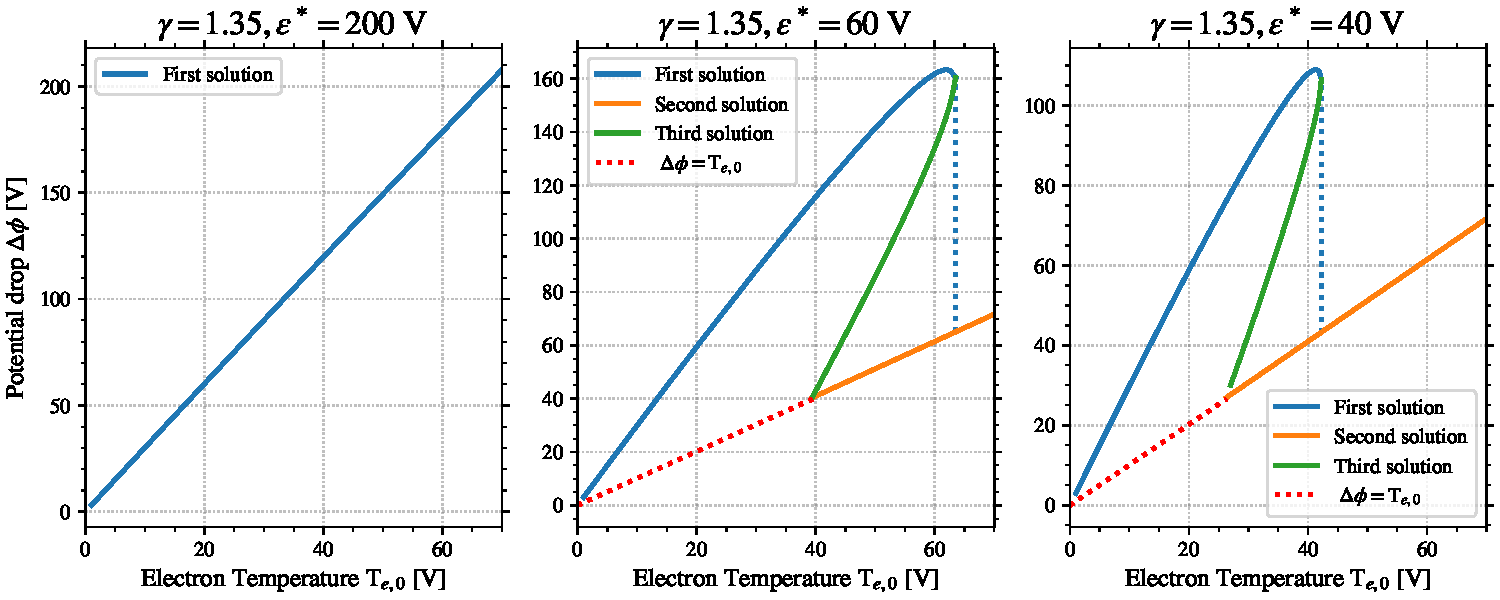
\includegraphics[width=\textwidth]{Potential_drop_poly_see.pdf}
  \caption{ Plasma potential drop to the wall as a function of the electron temperature for different values of the cross-over energy $\crover$ using \cref{eq-costseepoly}. It is the same results as  \cref{fig-dphivsTe} but with polytropic electron of index $\gamma=1.35$.}
  \label{fig-rso_crit_see}
\end{figure}

We observe in \cref{fig-rso_crit_see} that the electron temperature in the center $\Teb$ can be much higher before the inversion of the plasma sheath potential, compared to \cref{fig-dphivsTe}.
Indeed, the polytropic state law reduces the electron temperature at the wall, hence decreases the electron emission rate for a given $\Teb$.
Consequently, the electron bulk temperature can access higher temperature, compared to the one observed in \cref{fig-dphivsTe}.
Moreover, we see that the critical temperature for $\crover=40 \,\volt$ is close to $\Te=40\,\volt$, which is consistent with the transition between the regimes {\bf III} and {\bf II} observed in the \ac{PIC} simulations.

In addition, for some values of electron temperature, there are three solutions.
This could explain the oscillations observed in regime {\bf II}.
Indeed, when the electron temperature increases, the sheath follows the first solutions.
When the critical electron temperature is reached, the sheath jumps to the third solution.
It corresponds to the \ac{SCL} regime with an inverted sheath.
There, the electron temperature in the bulk decreases because of the increased electron power losses at the wall.
The electron temperature decreases until the second critical temperature, which corresponds to the moment when the third solution disappear, so that the sheath jumps back to the first solution.
We do not expect the third solution in-between to be observed in the simulations.

Obviously, the current model supposes that the polytropic index is constant.
However, we saw in the \ac{PIC} simulations that it increases from $\gamma = 1.34$ to $1.59$.
Hence, the exact values of the critical temperature may not exactly correspond to the one observed in the simulations.
On the other hand, we can expect the overall behavior not to be significantly affected.

\vspace{1em}
To summarize, the polytropic law is combined with electron emission to model the sheath.
The model obtained is richer than the usual isothermal model, as it allows multiple values of potential drop to the wall for the same electron bulk temperature.
This model only uses the electron bulk temperature and self-consistently computes both the potential drop and the electron emission rate.
It is compared in the next section to the \ac{PIC} simulation results.
